\section{Cross Section Evolution}
\label{sec:cross_sections}

We introduce a new method of origami construction, using cross section diagrams.
Instead of beginning our construction from a 2-dimensional sheet of paper, we
consider a 1-dimensional cross section moving forwards in time through 3D space.
A simple example using strip narrowing\cite{strip_narrowing} is demonstrated in
Figure~\ref{fig:strip_narrowing}.

\subsection{Segments and Cross Sections}
\label{sec:segments_and_cross_sections}

\begin{definition}
\label{def:segment}
A segment $s$ is an oriented line segment with left and right endpoints $\vec s_l$ and $\vec s_r$.
Each segment is also associated with an orientation vector $\vec{\hat o_s} \equiv\frac{\vec s_r-\vec s_l}{ \left\| \vec s_r-\vec s_l\right\|}$.
This vector serves to disambiguate the orientation of zero length segments.
\end{definition}

\begin{definition}
\label{def:cross_section}
A cross section $C$ is defined as an ordered list of line segments $\langle s_1,s_2,\cdots,s_n\rangle$,
such that for every segment $s_i$ (except the last),
the right endpoint of $s_i$ coincides with the left endpoint of $s_{i+1}$.
Each segment $s$ is also associated with a velocity vector $\vec{\hat v_s}$ of unit magnitude.
For a segment $s_i\in C$ we will also denote this velocity as $\vec{\hat v_i}$.
\end{definition}

\vspace{-1pc}
\begin{restatable}{inv}{UniformVelocity}
\label{inv:uniform_velocity}
All non-joint nodes on a segment $s$ have the same velocity $\vec{\hat v_s}$.
\end{restatable}
\vspace{-1pc}

\begin{restatable}{inv}{OrthogonalVelocity}
\label{inv:orthogonal_velocity}
The velocity $\vec{\hat v_s}$ of segment $s$ is orthogonal to its orientation $\vec{\hat o_s}$.
\end{restatable}

\begin{definition}
\label{def:node}
Given a cross section $C = \langle s_1, s_2,\cdots s_n \rangle$, a node $x$ denotes a point on one of the segments $s_i$.
A joint node is a node that resides on the endpoint of a segment.
The distance between two nodes on a cross section is defined as the overall length of cross section between the two nodes.
\end{definition}

\subsection{Joints}
\label{sec:joints}

\begin{definition}
\label{def:joints}
A cross section with $n$ segments is also associated with a list of joints
$ \langle J_1,\dots, J_{n-1} \rangle$,
where $\vec J_i$ corresponds to the right endpoint of $s_i$ (same as left endpoint of $s_{i+1}$.
A particular joint $\vec J_i$ is associated with a left segment $s_i$,
a right segment $s_{i+1}$, and a velocity $\vec J_v$.
\end{definition}

\begin{definition}
\label{def:joint_plane}
A joint plane is the plane that coincides with both segments $l$ and $r$ associated with a particular joint $J$.
In case the two segments are coincident (i.e. $\vec{\hat o}_l = \pm \vec{\hat o}_r$),
we define the joint plane to be orthogonal to $\vec{\hat v}_l = \vec{\hat v}_r$.
\end{definition}

\begin{definition}
\label{def:joint_plane_velocity}
Consider a joint $J$ associated with segments $l$, $r$, and joint plane $\mathcal P$,
where $\vec{\hat v}_l$ and $\vec{\hat v}_r$ are the velocities of segments $l$ and $r$.
We define $\vec{\hat v}_l^\shortparallel$ and $\vec{\hat v}_l^\perp$ as components of
$\vec{\hat v}_l$, such that $\vec{\hat v}_l^\shortparallel$ is the projection of $\vec{\hat v}_l$
onto $\mathcal P$, and $\vec{\hat v}_l^\perp = \vec{\hat v}_l - \vec{\hat v}_l^\shortparallel$
(orthogonal to $\mathcal P$).
Similarly, we define $\vec{\hat v}_r^\shortparallel$ and $\vec{\hat v}_r^\perp$, as the components of $\vec{\hat v}_r$.
By Invariant~\ref{inv:orthogonal_velocity}, $\vec{\hat v}_l^\shortparallel$ and $\vec{\hat v}_r^\shortparallel$
are orthogonal to $\vec{\hat o}_l$ and $\vec{\hat o}_r$ respectively.
This uniquely determines the direction of all velocity components.
\end{definition}

Henceforth, we will refer to the $\vec{\hat v}^\shortparallel$ component as the \emph{joint plane velocity},
and the $\vec{\hat v}^\perp$ component as the \emph{joint orthogonal velocity,}

\begin{restatable}{inv}{JointOrthogonalVelocity}
\label{inv:joint_orthogonal_velocity}
For a joint $J$ associated with segments $l$ and $r$, $\vec{\hat v}_l^\perp = \vec{\hat v}_r^\perp$
i.e. the joint orthogonal velocities have to be equal, such that the joint plane moves with a fixed velocity along it's normal.
As a corollary, $ \left\| \vec{\hat v}_l^\shortparallel\right\| = \left\| \vec{\hat v}_r^\shortparallel\right\|$.
\end{restatable}

\subsection{Time Travel}
\label{sec:time_travel}

In the process of time travel, all the nodes on a segment $s$,
except the \emph{joint nodes} move with velocity $\vec{\hat v_s}$ (orthogonal to $\vec{\hat o_s}$).
For example, if we allow a single segment of length $X$ to evolve for time $T$, it will result in a $X\times T$ strip of paper.

The joint node velocity $\vec J_v$ may have a component along a correspoding segment $s$ (along $\vec{\hat o_s}$).
As a result, the lengths of segments may change (Figure~\ref{fig:trapezoid_angles}).
This can be visualized as movement of the corresponding joint along one of the segments.

\begin{definition}
\label{def:segment_length}
For ever segment $s$ in a cross section $C$, we associate a left pace $L_s$,
which indicates the rate at which $s$ shrinks from its left endpoint.
Similarly, we define a right pace $R_s$ grows from its right endpoint.
Note that both these quantities can be negative.
\end{definition}
After time $T$, the length of a segment changes by $T\cdot(R_s-L_s)$.
The length of a segment is not allowed to become negative.
For a segment $s_i$ with left joint $J^L$ and right joint $J^R$, we obtain the relations
\begin{align}
\vec J_v^L-\vec{\hat v_{s_i}} = L_{s_i}\cdot \vec{\hat o_{s_i}} && \vec J_v^R-\vec{\hat v_{s_i}} = R_{s_i}\cdot \vec{\hat o_{s_i}}
\end{align}

\begin{proposition}
\label{prop:valid_joint}
A joint $J$ corresponding to segments $s$ and $t$ is \emph{valid} if and only if the evolution
resulting from the velocities $\vec{\hat v_l}$, $\vec{\hat v_r}$, and $\vec J_v$ preserves distances between nodes.
\end{proposition}
\begin{restatable}{pro}{LeftRightPace}
\label{pro:left_right_pace}
The right pace of $s_{i}$ is equal to the left pace of $s_{i+1}$.
This is to preserve the overall length of the cross section, and the distance between any two nodes.
Furthermore, the left pace of the first segment, and the right pace of the last segment should be zero, i.e. $L_0 = R_n = 0$
This ensures that the total length of the cross section does not change.
\end{restatable}

The movement of a joint increases the length of one of its associated segments,
and decreases the length of the other segment by the same amount (this ensures that the total length is preserved).
This puts some constraints on the possible velocities of adjacent segments.

%\begin{figure}[htpb]
\begin{wrapfigure}[12]{r}{0.5\textwidth}
\vspace{-2.2em}
\graphicspath{{./notebooks/}}
    \centering
    \def\svgwidth{0.5\textwidth}
    \input{notebooks/joint_plane_velocity.pdf_tex}
    \caption{A joint with segments $l$ and $r$.
    The trajectory of the joint is shown in orange.
    The trajectories of $a$ and $b$ are shown in blue.
    The green arrows indicate $\vec v^\shortparallel$}
    \label{fig:joint_plane_velocity}
\end{wrapfigure}
%\end{figure}

Consider a joint $\vec J_i$ corresponding to segments $l = s_i$ and $r = s_{i+1}$, at time $t=0$.
Henceforth, we will refer to $L_r$ as $L$, and $R_l$ as $R$.
Without loss of genenerality, we assume that $L<0$.
At a later time $t$, let the new joint position be $\vec J'_i$.
We define nodes $a$ and $b$ corresponding to $\vec J_i$ and $\vec J_{i+1}$ respectively.
We also define the initial and final positions of $a$ as $\vec a$,
and $\vec a'$, and similarly for $b$, we define $\vec b$ and $\vec b'$.
Let $d$ be the \emph{separation} between nodes $a$ and $b$.
this setup is shown in Figure~\ref{fig:joint_plane_velocity}

First, note that $\vec a, \vec b$ lie on the segment $l$, and $\vec a', \vec b'$ lie on the segment $r$,
which implies that $\vec b-\vec a = d\cdot \vec{\hat o_l}$, and $\vec b'-\vec a' = d\cdot \vec{\hat o_r}$.
\begin{align}
\vec b' - \vec a' &= (\vec b + t\cdot \vec{\hat v_r}^\shortparallel) - (\vec a + t\cdot \vec{\hat v_l}^\shortparallel)\\
\implies \vec b' - \vec a' &= (\vec b - \vec a) + t\cdot(\vec{\hat v_r}^\shortparallel - \vec{\hat v_l}^\shortparallel)\\
\implies d\cdot \vec{\hat o_r} &= d\cdot \vec{\hat o_l} + t\cdot(\vec{\hat v_r}^\shortparallel - \vec{\hat v_l}^\shortparallel)\\
\implies \vec{\hat v_r}^\shortparallel - \vec{\hat v_l}^\shortparallel &= \frac{d}{t}\cdot(\vec{\hat o_r}-\vec{\hat o_l})
= -R\cdot(\vec{\hat o_r}-\vec{\hat o_l}) = -L\cdot(\vec{\hat o_r}-\vec{\hat o_l})
\end{align}
This is only possible if $\vec{\hat o_l}\times \vec{\hat o_r}$ is oriented opposite to $\vec{\hat v_l}^\shortparallel\times \vec{\hat v_r}^\shortparallel$.

\begin{restatable}{pro}{SegmentOrientation}
\label{pro:SegmentOrientation}
Given two adjacent segments $l$ and $r$ in a cross section $C$, the vector
$\vec{\hat o_l}\times \vec{\hat o_r}$ must be oriented opposite to $\vec{\hat v_l}^\shortparallel\times \vec{\hat v_r}^\shortparallel$.
\end{restatable}

If the angle between the segments (between $\vec{\hat o_l}$ and $\vec{\hat o_r}$) is $\theta$,
the magnitude of $\vec{\hat o_r}-\vec{\hat o_l}$ is $\sqrt{2-2\cos(\theta)}$,
and $ \left\| \vec{\hat v_r}^\shortparallel-\vec{\hat v_l}^\shortparallel\right\| = v\cdot\sqrt{2-2\cos(\pi-\theta)}$.
Here, $v$ is magnitude of the plane velocity of $J_i$. Given $\phi = \theta/2$, we get --
\begin{align}
-L = -R &= \frac dt = \vec{\hat v_l} - \vec{\hat o_l}\frac{ \left\| \vec{\hat v_r}^\shortparallel
- \vec{\hat v_l}^\shortparallel\right\|}{ \left\| \vec{\hat o_r}-\vec{\hat o_l}\right\|}
&= v\cdot\frac{\sqrt{\sin^2\left( {\pi/2-\theta/2}\right)}}{\sqrt{\sin^2{\theta/2}}}
= v\cdot\cot\left( \phi \right)
\end{align}

\begin{restatable}{pro}{JointVelocity}
\label{pro:joint_velocity}
The velocity of a joint $J$ associated with segments $l$ and $r$, is a constant vector
$\vec J_v
%= \vec{\hat v_l} - \vec{\hat o_l}\frac{ \left\| \vec{\hat v_r}^\shortparallel
%- \vec{\hat v_l}^\shortparallel\right\|}{ \left\| \vec{\hat o_r}-\vec{\hat o_l}\right\|}
= \vec{\hat v_l} - \left\| \vec{\hat v_l}^\shortparallel\right\|\cdot\vec{\hat o_l}\cdot\cot\left( \theta/2 \right)$,
where $\theta$ is the angle between $\vec{\hat o_l}$ and $\vec{\hat o_r}$.
\end{restatable}

%\todo[inline]{
%Note that time evolution is reversible.
%}

\begin{figure}[htb]
\graphicspath{{./figures/}}
    \centering
    \subfloat[] {
        \def\svgwidth{0.5\textwidth}
        \input{figures/trapezoid.pdf_tex}
        \label{fig:segment_trapezoid}
    }
    \hspace{-9em}
    \subfloat[] {
        \def\svgwidth{0.7\textwidth}
        \input{figures/trapezoid_angles.pdf_tex}
        \label{fig:trapezoid_angles}
    }
    \caption{}
    \label{fig:trapezoids}
\end{figure}


\subsection{Cross Section Interval Folding}
\label{sec:interval_folding}

~
\vspace*{-4ex}

\begin{definition}
\label{def:interval}
We consider a cross section composed of segments $ \langle s_1,s_2,\cdots,s_n \rangle$
with total length $X$ (i.e., $\sum \left| s_i\right| = X$).
If we allow this cross section to evolve for time $T$, we obtain a new cross section $\langle r_1,r_2,\cdots ,r_n \rangle$.
The evolution forms a cross section interval $\mathcal C$ of length $T$.
The initial cross section is denoted as $\mathcal C_I = \langle s_1, s_2,\cdots s_n \rangle$,
and the final cross section is denoted as $\mathcal C_F = \langle r_1, r_2,\cdots r_n \rangle$.
\end{definition}

In this section, we focus on a single cross section interval $\mathcal C$ with segments $\langle s_1, s_2,\cdots s_n \rangle$ evolving over time $T$.
First consider the surface traced out by an individual segment $s_i$.
Since the endpoints of $s_i$ move in a straight line, each segment traces a trapezoid.
We define the \emph{height} of a trapezoid to be the distance between its parallel sides.

\begin{lemma}
\label{lem:trapezoid}
The surface traced out by a segment $s$ in time $T$ is a trapezoid $Z_s$ of height $T$ (Figure~\ref{fig:segment_trapezoid}).
Specifically, if $L,R$ are the initial left and right endpoints of $s$, and $L',R'$ are the final endpoints,
$Z_s = LL'R'R$ is the corresponding trapezoid (Figure~\ref{fig:segment_trapezoid}).
\end{lemma}
\begin{proof}
By Invariant~\ref{inv:joint_velocity}, we know that the joint trajectories are straight lines, which form the non-parallel sides.
Since the non-joint nodes on a segment all have the same velocity, the initial and final segment positions form the parallel sides.
\end{proof}

\begin{lemma}
\label{lem:trapezoid_gluing_parallel}
Consider a joint $J$ with segments $l$ and $r$,
which has zero orthogonal joint velocity (i.e., $\vec v_l^\perp = \vec v_r^\perp = \vec 0$).
The gluing of trapezoids $Z_l$ and $Z_r$ along the joint trajectory $\mathcal T_J$ is isometric to a larger trapezoid.
\end{lemma}
\begin{proof}
We consider the evolution of joint $J$ for time $T$ (Figure~\ref{fig:trapezoid_angles}).
First consider a coordinate system with $(\vec{\hat v}_l, \vec{\hat o}_l)$ as the basis.
Since, $\vec{\hat v}_l = \vec v_l^\shortparallel$, from Invariant~\ref{inv:joint_velocity},
we know that $-R_l = \left\| \vec v_l^\shortparallel\right\|\cdot\cot(\omega) = \cot(\omega)$.
So, $\vec J_v = \vec{\hat v}_l - \vec{\hat o}_v\cdot\cot(\omega)$.  Therefore,
\begin{align*}
    \cot(\angle LJJ') &= \frac{T\cdot R_l}{ \left\| T\cdot\vec{\hat v}_l\right\|} = \cot(\omega)
    \implies \angle LJJ' = \omega.
\end{align*}
Similarly, we consider a coordinate system with $(\vec{\hat v}_r, \vec{\hat o}_r)$ as the basis.
Since $\vec J_v = \vec{\hat v}_r - \vec{\hat o}_r\cdot \cot(\omega)$, we get
$$
\cot(\angle RJJ') = \frac{-\left\| T\cdot L_r\right\|}{ \left\| T\cdot(\vec J_v - L_r)\right\|} = -\cot(\omega)
\implies \angle RJJ' = \pi - \omega.
$$
This implies that $\cot(\angle RJJ') + \cot(\angle LJJ') = \pi$.
So, the gluing of $Z_l$ and $Z_r$ along the joint trajectory $JJ'$ is isometric to a larger trapezoid.
\end{proof}

\begin{figure}[!htb]
\graphicspath{{figures/trapezoidZ}}
    \centering
    %\subfloat[]{
        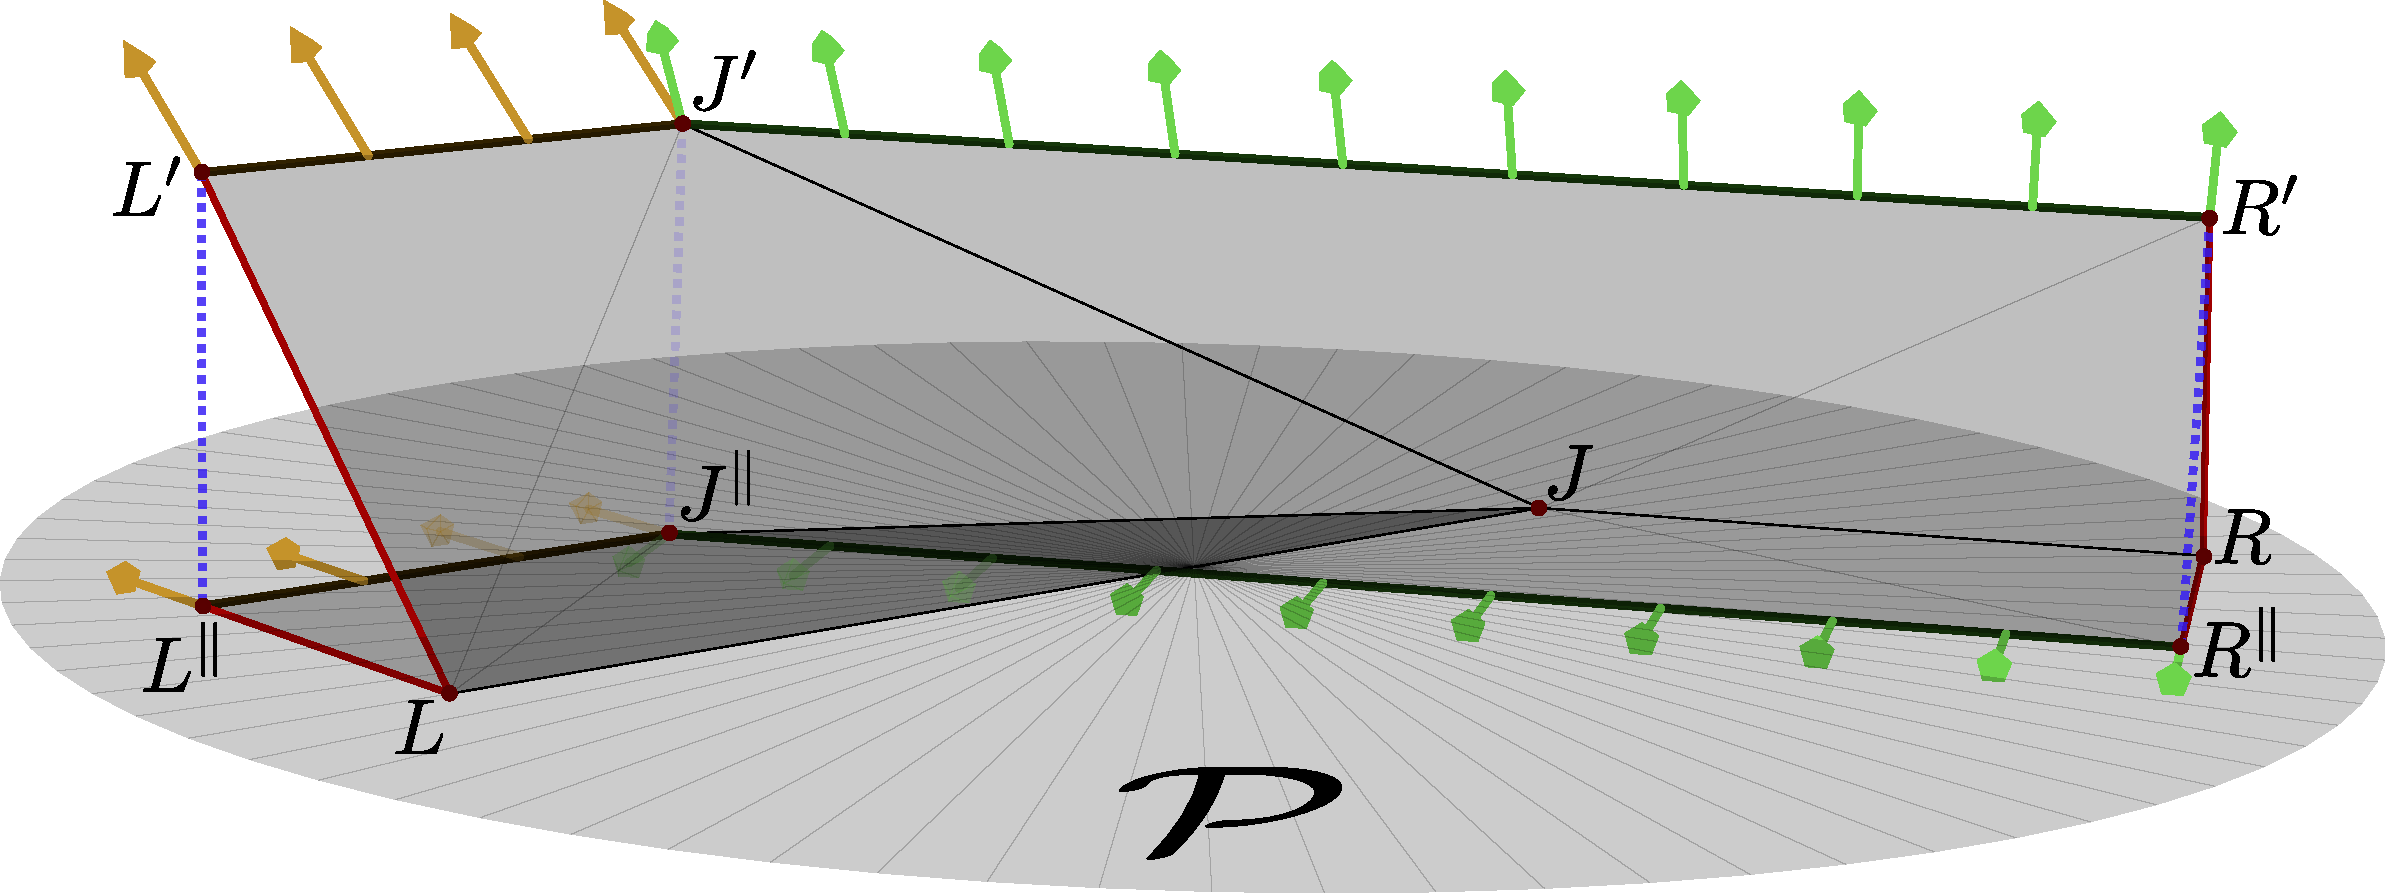
\includegraphics[width=0.5\textwidth]{figures/trapezoidZ/trapezoidZ0.pdf}%
    %}%
    %\subfloat[]{
        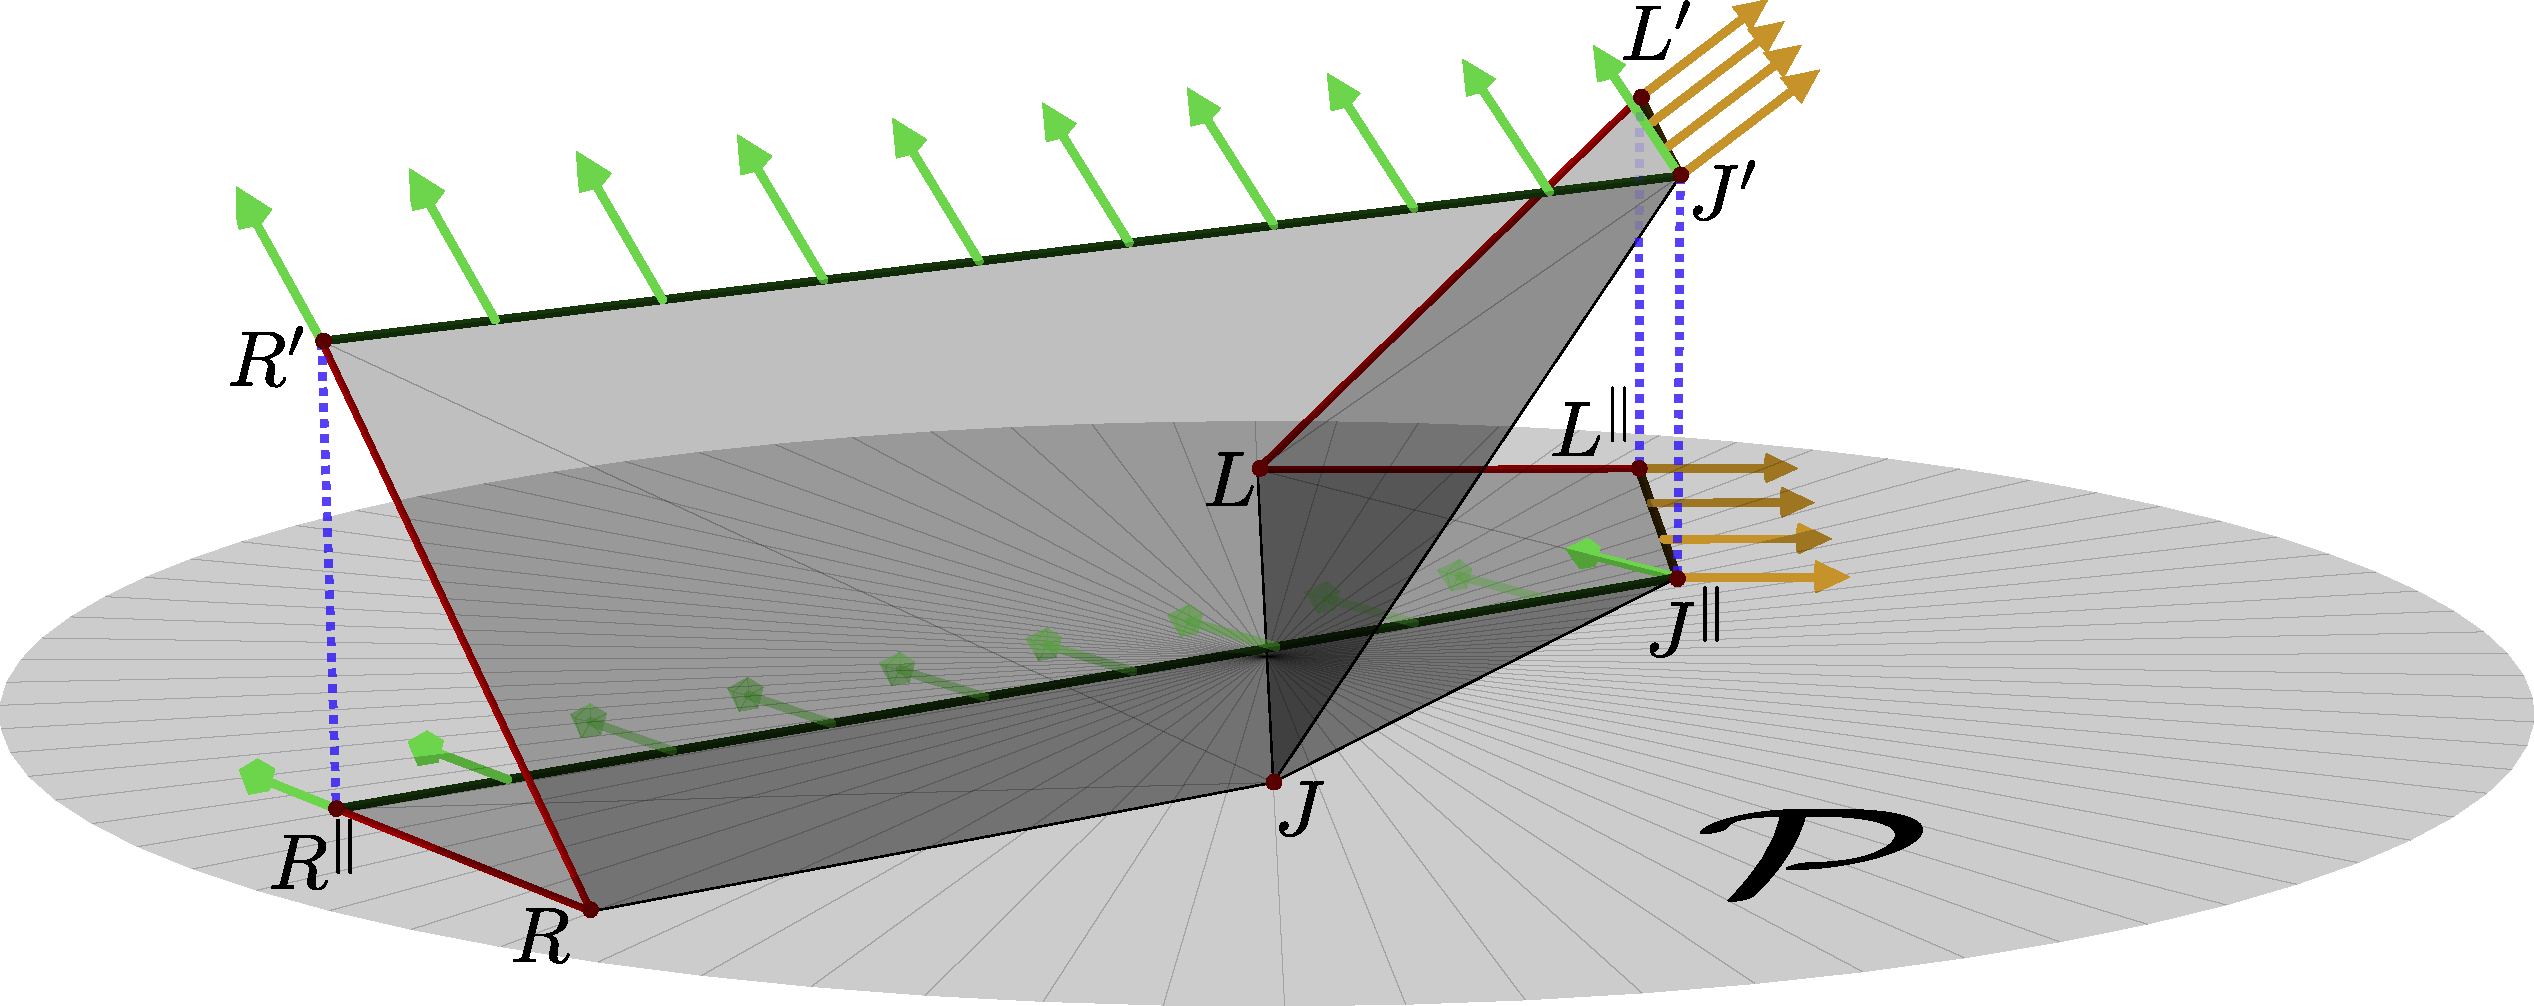
\includegraphics[width=0.5\textwidth]{figures/trapezoidZ/trapezoidZ1.pdf}%
    %}%

    %\subfloat[]{
        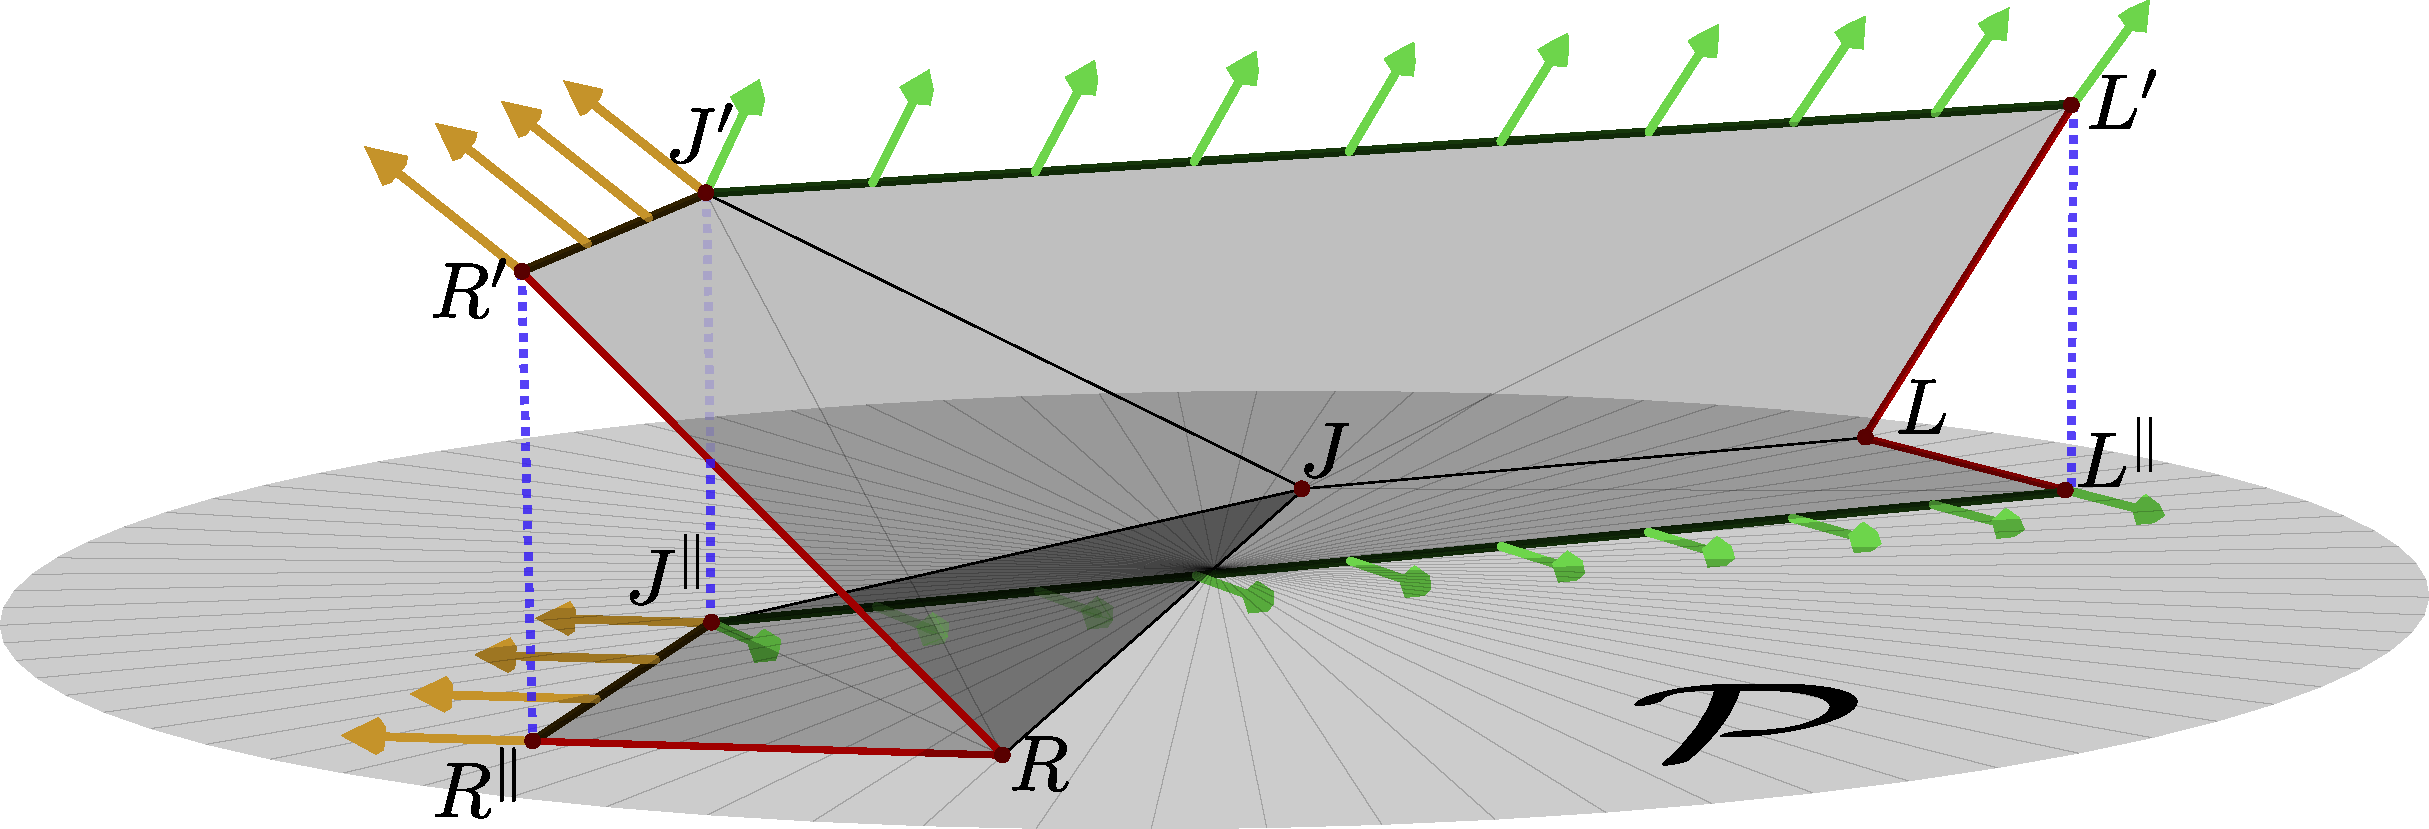
\includegraphics[width=0.8\textwidth]{figures/trapezoidZ/trapezoidZ2.pdf}%
    %}%
    \caption{
    Evolution of a joint with non-zero orthogonal velocity from $LJR$ to $L'J'R'$.
    The blue dotted lines represent the projection of the final state to the joint plane $\mathcal P$.
    }
    \label{fig:trapezoidZ}
\end{figure}


~
\vspace*{-4ex}

\begin{lemma}
\label{lem:trapezoid_gluing}
Consider a joint $J$ with segments $l$ and $r$ with non-zero orthogonal velocity; see Figure~\ref{fig:trapezoidZ}.
The gluing of trapezoids $Z_l$ and $Z_r$ along the joint trajectory $\mathcal T_J$ is isometric to a larger trapezoid.
\end{lemma}

\begin{proof}
As before, let $LJR$ and $L'J'R'$ represent the initial and final positions of the segments respectively.
We also construct the projection of $L'J'R'$ to the joint plane $\mathcal P$ as $L^\shortparallel J^\shortparallel R^\shortparallel$.
The evolution of the projection is analogous to the setting in Lemma~\ref{lem:trapezoid_gluing_parallel}.
Therefore, $\angle LJJ^\shortparallel = \omega = \theta/2$ and $\angle RJJ^\shortparallel = \pi-\omega$.

Consider the positive $z$-axis along the joint orthogonal velocity (i.e., normal to the joint plane $\mathcal P$).
We define the orthogonal displacement vector as $\overrightarrow{JJ'} = z\cdot\vec{\hat k}$.
Let the positive $x$-axis be along $JJ^\shortparallel$. So, the unit vector along $\overrightarrow{JJ'}$ is $\frac{1}{\sqrt{1+z^2}}(1,0,z)$.

Since $\angle J^\shortparallel JR = \omega$, the unit vector along $\overrightarrow JR$ is $(\cos\omega,\sin\omega,0)$.
So, we compute $\cos \angle RJJ' = \cos\omega/\sqrt{1+z^2}$.
Similarly, since $\angle J^\shortparallel JL = \pi-\omega$, the unit vector along $\overrightarrow JL$ is $(-\cos\omega,\sin\omega,0)$,
which implies that $\cos \angle LJJ' = -\cos\omega/\sqrt{1+z^2}$.
Finally, since both $\angle LJJ$ and $\angle RJJ'$ are less than $\pi$, and $\cos\left(\angle LJJ' \right) = -\cos\left(\angle RJJ' \right)$,
we conclude that $\angle LJJ' + \angle RJJ' = \pi$.
Since $LJJ'L'$ and $RJJ'R'$ are both trapezoids, this implies that the resulting gluing along $JJ'$ is isometric to a larger trapezoid.
\end{proof}

\begin{definition}
\label{def:interval_folding}
Consider a cross section interval $\mathcal C$ formed from a cross section $C$ evolving over time $T$.
By Lemma~\ref{lem:trapezoid}, the segments $ \langle s_1, s_2,\cdots s_n \rangle$ form trapezoids
$ \langle Z_1, Z_2,\cdots Z_n \rangle$ each of height $T$, where $Z_i$ represents the $i^{th}$ trapezoid in folded space.
The folding (the final folded state) $\mathcal F_C^T$ corresponding to $\mathcal C$ is formed by successively gluing the trapezoids
$Z_i$ to $Z_{i+1}$ along the trajectory of joint $\vec J_i$ (for $1\le i<n$) to form a connected shape.
\end{definition}

\begin{definition}
\label{def:interval_folding_boundary}
Given a cross section interval $\mathcal C$ with folding $\mathcal F_C^T$,
the initial-boundary of a folding $\mathcal F_C^T$ is defined as the union of the initial cross section segments in $\mathcal C_I$,
where the right endpoint of the $i$th segment is attached to the left endpoint of the $(i+1)$st segment.
Similarly, the final-boundary of $\mathcal F_C^T$ is defined as the union of the final segments in $\mathcal C_F$.
\end{definition}

\begin{restatable}{thm}{interval_strip}
\label{thm:interval_strip}
Consider a cross section interval $\mathcal C$ formed from a cross section $C$ evolving over time $T$ to form a folding $\mathcal F_C^T$.
Further assume that the total length of cross section $C$ is $X$ units. Then, $\mathcal F_C^T$ is isometric to a $X\times T$ strip of paper.
\end{restatable}
\begin{proof}
By repeated use of Lemma~\ref{lem:trapezoid_gluing}, we know that $\mathcal F_C^T$ is isometric to a trapezoid.
Let $L,L'$ be the initial and final positions of the left (non-parallel) edge of the trapezoid, and
let $R,R'$ be the initial and final positions of the right edge of the trapezoid.
Say that $C$ comprises of segments $ \langle s_1, s_2,\cdots s_n \rangle$.
From Invariant~\ref{inv:left_right_pace}, we know that the left pace of $s_0$ is zero.
So, the line $LL'$ follows the trajectory of $\vec{\hat v_0}$, which is orthogonal to the segment $s_0$.
In other words, the left edge of the trapezoid has length $T$, and is orthogonal to the parallel edges.
Similarly, because the right pace of $s_n$ is zero, the right edge of the trapezoid is also orthogonal.
Therefore, $\mathcal F_C^T$ is isometric to a right angled trapezoid (i.e., a strip) of length $X$ and width $T$.
\end{proof}

\begin{remark}
\label{rem:joint_crease}
The trajectory of a joint forms a crease in the folded state.
\end{remark}

\subsection{Multiple Cross Sections}
\label{sec:intervals}

\begin{definition}
\label{def:compatible}
Given two cross section intervals $\mathcal C$ and $\mathcal D$, such that $\mathcal C_F$ and $\mathcal D_I$ are equivalent,
we say that $\mathcal D$ is next-compatible with $\mathcal C$ and $\mathcal C$ is previous-compatible with $\mathcal D$.
Two cross sections $C = \langle s_1, s_2,\cdots s_n \rangle$ and $D = \langle r_1, r_2,\cdots r_m \rangle$ are equivalent
if and only if $C$ and $D$ correspond to the same sequence of segments after the deletion of all zero length segments.
\end{definition}

\begin{definition}
\label{def:cross_section_sequence}
A cross section sequence is a sequence is an ordered list of cross section intervals
$ \langle \mathcal C_1, \mathcal C_2,\cdots \mathcal C_n \rangle$,
such that $C_{i}$ is next-compatible with $C_{i-1}$ for all $i\in [n-1]$.
This is equivalent to stating that $C_{i}$ is previous-compatible with $C_{i+1}$ for all $i\in [n-1]$.
Note that we do not care about the velocities of the segments.
\end{definition}

We will represent our full construction as a valid \emph{cross section sequence}.
Given a cross section sequence $\langle \mathcal C_1, \mathcal C_2,\cdots \mathcal C_n \rangle$,
the transition from $\mathcal C_i$ to $\mathcal C_{i+1}$ corresponds to the deletion of one or more
length zero segments from $\mathcal C_i$, and the addition of one or more zero length segments to obtain $\mathcal C_{i+1}$.
Figure~\ref{fig:strip_narrowing} shows a simple example.
\graphicspath{{./figures/strip_narrowing/}}
\begin{figure}[]
    \centering
    \begingroup
    \def\svgwidth{0.21\textwidth}
        \captionsetup[subfigure]{width=0.22\textwidth}
        \subfloat[The trivial cross section.]{\centering
        \input{figures/strip_narrowing/strip0.pdf_tex}
        }%
    \endgroup
    \hfill
    \begingroup
    \def\svgwidth{0.21\textwidth}
        \captionsetup[subfigure]{width=0.48\textwidth}
        \subfloat[New zero length segment inserted at left endpoint. Existing segment reverses velocity.]{\centering
        \input{figures/strip_narrowing/strip10.pdf_tex}
        %}%
    %\endgroup%
    %\begingroup
    \def\svgwidth{0.21\textwidth}
        %\captionsetup[subfigure]{width=0.22\textwidth}
        %\subfloat[] {
        \input{figures/strip_narrowing/strip11.pdf_tex}
        }%
    \endgroup
    \hfill
    \begingroup
    \def\svgwidth{0.21\textwidth}
        \captionsetup[subfigure]{width=0.24\textwidth}
        \subfloat[Evolution continues]{%
          \makebox[0.24\textwidth]{\input{figures/strip_narrowing/strip12.pdf_tex}}
        }%
    \endgroup%

    \vspace{-1.2em}

    \begingroup
    \def\svgwidth{0.21\textwidth}
        \captionsetup[subfigure]{width=0.67\textwidth}
        \subfloat[New zero length segment (red) inserted between two existing segments
                  with the same velocity as the rightmost segment.
                  Existing segments retain their velocites.] {
        \input{figures/strip_narrowing/strip20.pdf_tex}
        %}%
    %\endgroup%
    %\begingroup
    \def\svgwidth{0.21\textwidth}
        %\captionsetup[subfigure]{width=0.22\textwidth}
        %\subfloat[] {
        \input{figures/strip_narrowing/strip21.pdf_tex}
        %}%
    %\endgroup%
    %\begingroup
    \def\svgwidth{0.21\textwidth}
        %\captionsetup[subfigure]{width=0.22\textwidth}
        %\subfloat[] {
        \input{figures/strip_narrowing/strip22.pdf_tex}
        }%
    \endgroup%
    %\begingroup
    %\def\svgwidth{0.21\textwidth}
        %\captionsetup[subfigure]{width=0.22\textwidth}
        %\subfloat[Evolution continues] {
        %\input{figures/strip_narrowing/strip23.pdf_tex}
        %}%
    %\endgroup%
    \hfill
    \begingroup
    \def\svgwidth{0.21\textwidth}
        \captionsetup[subfigure]{width=0.28\textwidth}
        \subfloat[Length of leftmost (blue) segment becomes zero.]{%
          \makebox[0.28\textwidth]{\input{figures/strip_narrowing/strip24.pdf_tex}}
        }%
    \endgroup%

    \vspace{-1.2em}

    \begingroup
    \def\svgwidth{0.21\textwidth}
        \captionsetup[subfigure]{width=0.47\textwidth}
        \subfloat[Leftmost (zero length) segment is deleted.
                  The remaining two segments continue in the same direction.
                  Overall strip width has been reduced] {
        \input{figures/strip_narrowing/strip30.pdf_tex}
        %}%
    %\endgroup%
    %\begingroup
    \def\svgwidth{0.21\textwidth}
        %\captionsetup[subfigure]{width=0.22\textwidth}
        %\subfloat[] {
        \input{figures/strip_narrowing/strip31.pdf_tex}
        }%
    \endgroup%
    \hspace{1.5em}
    \begingroup
    \def\svgwidth{0.42\textwidth}
        \captionsetup[subfigure]{width=0.42\textwidth}
        \subfloat[Side view of strip narrowing gadget, with layers separated. The red lines denote the boundaries of the cross section.] {
        \input{figures/strip_narrowing/strip_layers.pdf_tex}
        }%
    \endgroup%
        \caption{Cross section evolution of a strip narrowing gadget \cite{strip_narrowing}.}
    \label{fig:strip_narrowing}
\end{figure}


\begin{definition}
\label{def:sequence_folding}
Given a cross section sequence $\langle \mathcal C_1, \mathcal C_2,\cdots \mathcal C_n \rangle$,
We obtain $\mathcal F_i^T$ as the folding of cross section $\mathcal C_i$.
For each $i\le n-1$, we attach $\mathcal F_i^T$ to $\mathcal F_{i+1}^T$ by gluing
the final cross section of $\mathcal C_i$ to the initial cross section of $\mathcal C_{i+1}$.
This results in the final folding of the cross section sequence.
\end{definition}

\begin{proposition}
\label{prop:creases}
In addition to the creases formed along the trajectory of joints (Remark~\ref{rem:joint_crease}),
creases are also created when a segment changes velocity.
For instance, consider two adjacent cross sections $\mathcal C$ and $\mathcal D$,
with corresponding segments $s_C\in \mathcal C_F$ and $s_D\in \mathcal D_I$,
where $s_C$ and $s_D$ are identical except for their velocity direction.
Then, the segment $s_C$ (same as $s_D$) forms a crease in the folded state.
\end{proposition}

\subsubsection{Evolution Corresponds to Flat Paper}
\label{sec:flat}

In this section we will demonstrate that the folding formed by cross section evolution is realizable from a sheet of flat paper.
We note here that our construction may still result in self intersections.

We consider a cross section sequence $\langle \mathcal C_1, \mathcal C_2,\cdots \mathcal C_n \rangle$,
where each cross section interval $\mathcal C_i$ has evolution time $T_i$.
We then use Theorem~\ref{def:cross_section_sequence} to attach the sequence of $X\times T_i$ strips,
to form a complete $X\times T$ sheet of paper, where $T = \sum T_i$.

\begin{restatable}{thm}{main}
\label{thm:main}
Consider a cross section sequence $\mathcal C = \langle \mathcal C_1, \mathcal C_2,\cdots \mathcal C_m \rangle$ where each
cross section interval $\mathcal C_i$ evolves over time $T_i$ to form a folding $\mathcal F_i$
such that Invariants~1-6 hold for all segments and joints in each of the cross sections involved.
%\begin{itemize}
    %\item[] \vspace{-1.6em}\UniformVelocity*
    %\item[] \vspace{-1.6em}\OrthogonalVelocity*
    %\item[] \vspace{-1.6em}\JointOrthogonalVelocity*
    %\item[] \vspace{-1.6em}\LeftRightPace*
    %\item[] \vspace{-1.6em}\SegmentOrientation*
    %\item[] \vspace{-1.6em}\JointVelocity*
%\end{itemize}
Then, the folding $\mathcal F_{\mathcal C}$ obtained by successively gluing the final boundary of $\mathcal F_i$ to the initial boundary
of $\mathcal F_{i+1}$ (for each $1\le i<m$), is isometric to a $X\times T$ strip of paper, where $T = \sum T_i$.
\end{restatable}
\begin{proof}
From Theorem~\ref{thm:interval_strip}, we know that each $\mathcal F_i$ is isometric to a strip $Z_i$ of size $X\times T_i$.
Further, the initial and final cross sections of $\mathcal C_i$ form the parallel sides of $Z_i$ (of length $X$).
The gluing of $n$ strips of size $X\times T_i$ forms a strip of size $X\times T$.
So, the final folding is isometric to a sheet of paper with size $X\times T$.
\end{proof}

%\subsection{Evolution Corresponds to Flat Paper}
\label{sec:flat}

In this section we wil demonstrate that the folding formed by cross section evolution is realizable from a sheet of flat paper.
We note here that our construction may still result in self intersections.

We consider a cross section sequence $\langle \mathcal C_1, \mathcal C_2,\cdots \mathcal C_n \rangle$,
where each cross section interval $\mathcal C_i$ has evolution time $T_i$.
Say that the length ogf each cross section in the sequence is $X$.
We will denote a strip of paper of size $X\times L$ as an $L$-strip.

First, we will show that each $\mathcal C_i$ corresponds to a $T_i$-strip.
We will then use Theorem~\ref{def:cross_section_sequence} to attach the sequence of $T_i$-strips,
to form a complete $X\times T$ sheet of paper, where $T = \sum T_i$.

\subsubsection{Cross Section Interval Forms a Strip from a Gluing of Trapezoids}
\label{sec:cross_section_interval_strip}

In this section, we focus on a single cross section interval $\mathcal C$ with segments $\langle s_1, s_2,\cdots s_n \rangle$ evolving over time $T$.
First consider the surface traced out by an individual segment $s_i$.
Since the endpoints of $s_i$ move in a straight line, each segment traces \todo{What is a trace?} a trapezoid.

\begin{figure}[htb]
\graphicspath{{./figures/}}
    \centering
    \subfloat[] {
        \def\svgwidth{0.5\textwidth}
        \input{figures/trapezoid.pdf_tex}
        \label{fig:segment_trapezoid}
    }
    \hspace{-9em}
    \subfloat[] {
        \def\svgwidth{0.7\textwidth}
        \input{figures/trapezoid_angles.pdf_tex}
        \label{fig:trapezoid_angles}
    }
    \caption{}
    \label{fig:trapezoid}
\end{figure}

\begin{definition}
\label{def:trapezoid}
The surface traced out by a segment $s$ is a trapezoid $Z_s$ (Figure~\ref{fig:segment_trapezoid}).
Specifically, if $L,R$ are the initial left and right endpoints of $s$, and $L',R'$ are the final endpoints,
$Z_s = LL'R'R$ is the corresponding trapezoid (Figure~\ref{fig:segment_trapezoid}).
\end{definition}

\todo[inline]{Define gluing}

\begin{lemma}
\label{lem:trapezoid_gluing_parallel}
Consider a joint $J$ with segments $l$ and $r$, which has zero orthogonal joint velocity (i.e. $\vec v_l^\shortparallel = \vec v_r^\shortparallel = 0$.
The gluing of trapezoids $Z_l$ and $Z_r$ along the joint trajectory $\mathcal T_J$ is isometric to a larger trapezoid.
This joint trajectory is actually nothing but a crease in the folded state.
\end{lemma}

\begin{lemma}
\label{lem:trapezoid_gluing}

\end{lemma}


\begin{theorem}
\label{thm:cross_section_interval_strip}
The resulting gluing from any given cross section interval $\mathcal C$ with evolution time $T$ is isometric to a $T$-strip.
\end{theorem}


\subsubsection{Gluing the Interval Strips Together}
\label{sec:interval_strip_gluing}



